\documentclass[11pt,a4paper]{report}

\usepackage[utf8]{inputenc}
\usepackage[english]{babel}
\usepackage[english]{isodate}
\usepackage[parfill]{parskip}

\usepackage{graphicx}
%%
% Just some sample text
\usepackage{lipsum}
\usepackage{tabularx}
\usepackage{xcolor} % for colour
\usepackage{colortbl}
%\usepackage{multirow}
\usepackage{lettrine}

\usepackage{amsmath}
\usepackage{mathtools}
\usepackage{amssymb}
\usepackage{nccmath}
\usepackage{relsize}
\usepackage{eurosym}


\begin{document}


\begin{figure}
	\centering
	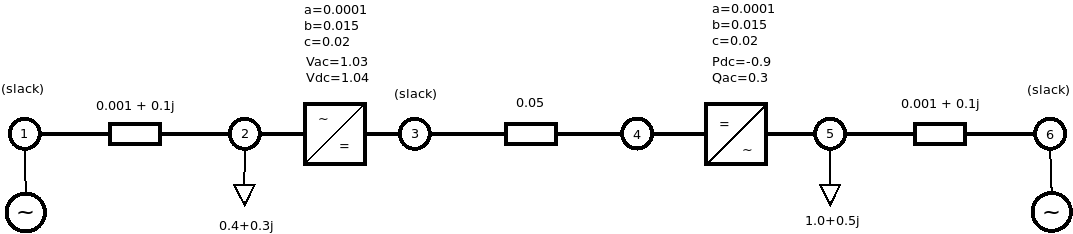
\includegraphics[width=0.99\linewidth]{acdc_6bus_diagram}
	\caption{}
	\label{fig:acdc6busdiagram}
\end{figure}

\begin{equation}
	\begin{bmatrix}
		\frac{\partial P}{\partial \theta} & \frac{\partial P}{\partial V_m} & \frac{\partial P}{\partial P_f} & \frac{\partial P}{\partial P_t} & \frac{\partial P}{\partial Q_t}\\
		\frac{\partial Q}{\partial \theta} & \frac{\partial Q}{\partial V_m} & \frac{\partial Q}{\partial P_f} & \frac{\partial Q}{\partial P_t} & \frac{\partial Q}{\partial Q_t}\\
		\frac{\partial P_{conv}}{\partial \theta} & \frac{\partial P_{conv}}{\partial V_m} & \frac{\partial P_{conv}}{\partial P_f} & \frac{\partial P_{conv}}{\partial P_t} & \frac{\partial P_{conv}}{\partial Q_t}\\
	\end{bmatrix}	
	\times 
	\begin{bmatrix*}[l]
		\Delta \theta  \quad \forall \ i_{pv} \cup i_{pq}   \\
		\Delta V_m     \quad \forall \ i_{pq}  \\
		\Delta P_f     \quad \forall \ k_{conv} \\
		\Delta P_t     \quad \forall \ k_{conv} \\
		\Delta Q_t     \quad \forall \ k_{conv}
	\end{bmatrix*}
	= 
	\begin{bmatrix*}[l]
		\Delta P \quad \ \ \forall \ i_{pv} \cup i_{pq} \\
		\Delta Q \quad \ \ \forall \ i_{pq}  \\
		\Delta P_{conv} \quad \forall \ k_{conv} 
	\end{bmatrix*}
\end{equation}


Active power nodal balance:
\begin{equation}
	\Delta P = P^{calc} - P^{esp}
\end{equation}


Reactive power nodal balance:
\begin{equation}
	\Delta Q = Q^{calc} - Q^{esp}
\end{equation}


Converter power balance:
\begin{equation}
	\Delta P_{conv} = P_f + P_t - P_{loss}
\end{equation}

In this equation $P_f$ and $P_t$ are variables to be found iteratively.

\end{document}